\documentclass[aspectratio=169]{beamer}
\usetheme{Madrid}
\usepackage[utf8]{inputenc}
\usepackage[T1]{fontenc}
\usepackage{tikz}
\usepackage{amssymb}
\usepackage{graphicx}
\setbeamertemplate{navigation symbols}{}
\setbeamercolor{title}{fg=white,bg=orange!85!red}
\setbeamercolor{frametitle}{fg=white,bg=orange!85!red}
\setbeamercolor{block title}{bg=orange!85!red!20,fg=black}
\setbeamercolor{block body}{bg=orange!85!red!8,fg=black}
\setbeamercolor{item}{fg=orange!85!red}
\setbeamercolor{itemize item}{fg=orange!85!red}
\setbeamertemplate{itemize item}[triangle]

\title{Block Arcade 4 — Variables}
\subtitle{Score and lives — numbers the game tracks and shows the player}
\author{ByteForge --- Grade 7 --- Game Maker}
\date{}

\begin{document}

\begin{frame}
    \titlepage
\end{frame}

\begin{frame}{Today's Plan}
    \begin{itemize}
        \item Score Counter
        \item Score Goes Up
        \item[$\bigstar$] BOSS --- Score \& Lives HUD
    \end{itemize}
\end{frame}

\begin{frame}{A variable the PLAYER can see}
    \large
    \begin{itemize}
        \item A score no one can see isn't really a score to the player
        \item Drawing it every frame turns an internal number into a real scoreboard.
    \end{itemize}
\end{frame}


\begin{frame}{Redrawing every frame keeps the display current}
    \large
    \begin{itemize}
        \item Because the display re-reads the variable fresh every frame, it always shows whatever score currently IS.
    \end{itemize}
\end{frame}


\begin{frame}{BOSS — a real two-stat HUD}
    \large
    \begin{itemize}
        \item Score AND lives, shown together, is genuinely what almost every simple arcade game's display actually is.
    \end{itemize}

    \begin{center}
    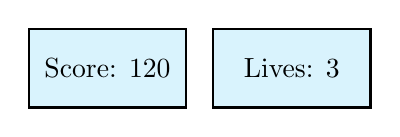
\begin{tikzpicture}[scale=0.9]

        \node[draw, thick, fill=cyan!15, minimum width=2cm, minimum height=1cm] at (0,0) {Score: 120};
        \node[draw, thick, fill=cyan!15, minimum width=2cm, minimum height=1cm] at (2.6,0) {Lives: 3};
    \end{tikzpicture}
    \end{center}
\end{frame}

\begin{frame}{Real-World Examples}
    \large
    \begin{itemize}
        \item Any arcade game's top-of-screen HUD (score, lives, timer)
        \item Point at three different real games' HUDs and identify which numbers are tracked as variables. Minecraft's hotbar (which item is selected), hunger bar, and health hearts are all live variables displayed every frame, exactly like this chapter's HUD.
    \end{itemize}
\end{frame}


\begin{frame}{Image}
    \begin{center}
    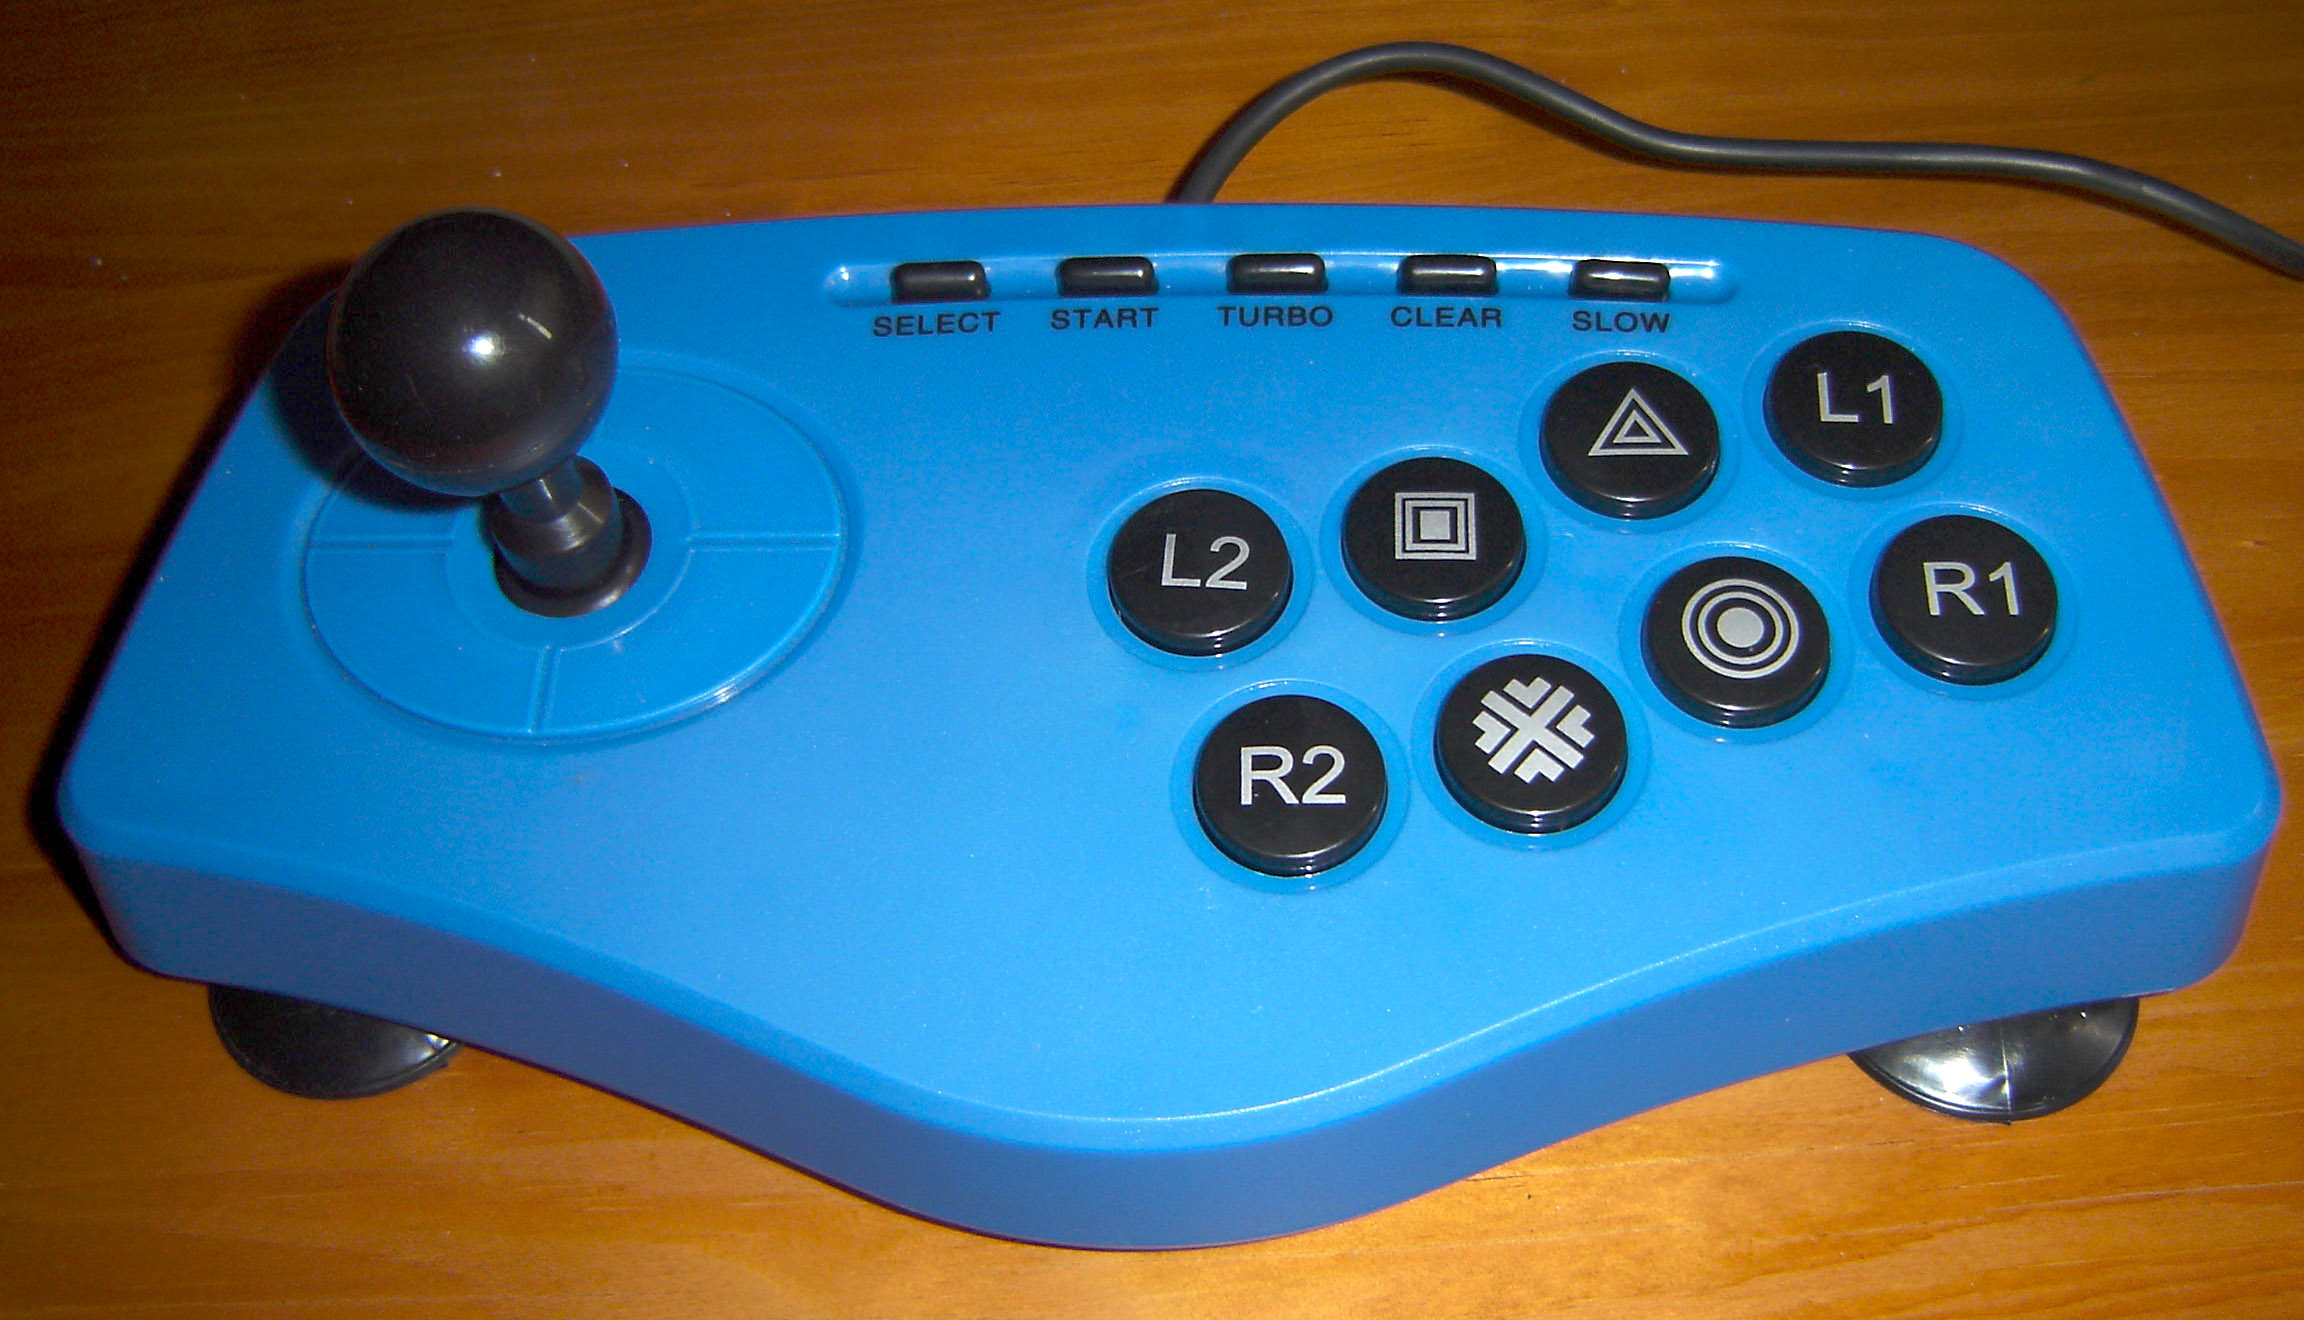
\includegraphics[width=0.5\textwidth]{images/arcade.jpg}

    \large A real HUD --- score and lives --- on a real arcade cabinet.

    \small Arcade controller — Carioca, CC BY-SA 3.0, via Wikimedia Commons
    \end{center}
\end{frame}

\begin{frame}{Let Them Discover}
    \Large
    Screenshot or sketch three different games' HUDs (including Minecraft's). What numbers do they ALL show? What's unique to just one of them (a timer, ammo count, a combo multiplier, Minecraft's armor bar)?
\end{frame}

\begin{frame}{Your Turn}
    \Large
    Open the student map, find \textbf{Block Arcade 4 — Variables}, and work through it
    hands-on --- everything you just saw, they now do themselves.
\end{frame}

\end{document}
